\documentclass[a4paper,12pt]{article}

\usepackage[brazilian]{babel}
\usepackage[utf8]{inputenc}
\usepackage[T1]{fontenc}

\title{MAC0211 - Laboratório de Programação I - Relatorio Jogo}	
\author{Felipe Tulio, Guilherme F. Silva, Marcos Kazuya}	

\usepackage{graphicx}  

\begin{document}
\maketitle
\section {Introdução}

			
Projeto Tamarindo.
 
Duas famílias muito unidas e poderosas sonham em ver seus apaixonados herdeiros, o príncipe
Teodoro e a princesa Dalila, unidos pelo casamento. Essa união vai garantir a força
e estabilidade do reino por muitas gerações.

Mas esse amor é ameaçado por outros dois reinos, que desejam impedir que essa união se concretize para terem para si o poder da familia da princesa. Para isso, os lordes bloquearam todos os possíveis caminhos na tentativa de impedir esse matrimônio.

Todavia, não puderam impedir a passagem pelo grande de rio que se localizava entre os quatro reinos. Tentando diminuir as possibilidades dessa travessia, os lordes reuniram seus exércitos e como arma secreta, e convocaram os mais poderosos magos em suas terras.


O herói, sabendo que o único meio possível de conseguir encontrar sua amada era tentar atravessar o rio, ordenou que os melhores artesãos construíssem um barco, este muito resistente, e ainda contou com a ajuda do antigo feiticeiro do castelo para essa jornada. E a partir desse ponto a história do nosso começa...

\section {Objetivo}

Atravessar o rio sem encostar nos navios, bombas, tubarão, fantasma, polvos e dragões afim de encontrar o castelo onde a princesa mora.


\section {Controles}
\subsection{Acelera}
$\uparrow$ acelera o barco; 

\subsection{Ré}
$\downarrow$ faz o barco dar ré;

\subsection{Esquerda}
$\leftarrow$ gira o barco 45 graus no sentido anti-horário;

\subsection{Direita}
$\rightarrow$ gira o barco 45 graus no sentido horário;

\subsection{Música}
M para ou inicia a Música.

\section {O jogo}
Composto por quatro fases por onde o principe deve passar, cada um com um nivel de dificuldade diferente, na primeira ele deve atravessar o rio que esta sendo bombardeado por navios inimigos, na segunda o rio esta repleto de tubarões e polvos gigantes, na terceira por fantasmas e navios amaldiçoados e na quarta e ultima onde esta o castelo da princesa há dragões pelo mapa.

Ao inicio de cada fase você recebe três vidas para tentar avançar de cenário. Se você falhar ao obter a vitória, você perde.

Ao tocar um inimigo, você perde uma vida.


\begin{figure}  
\begin{center}  
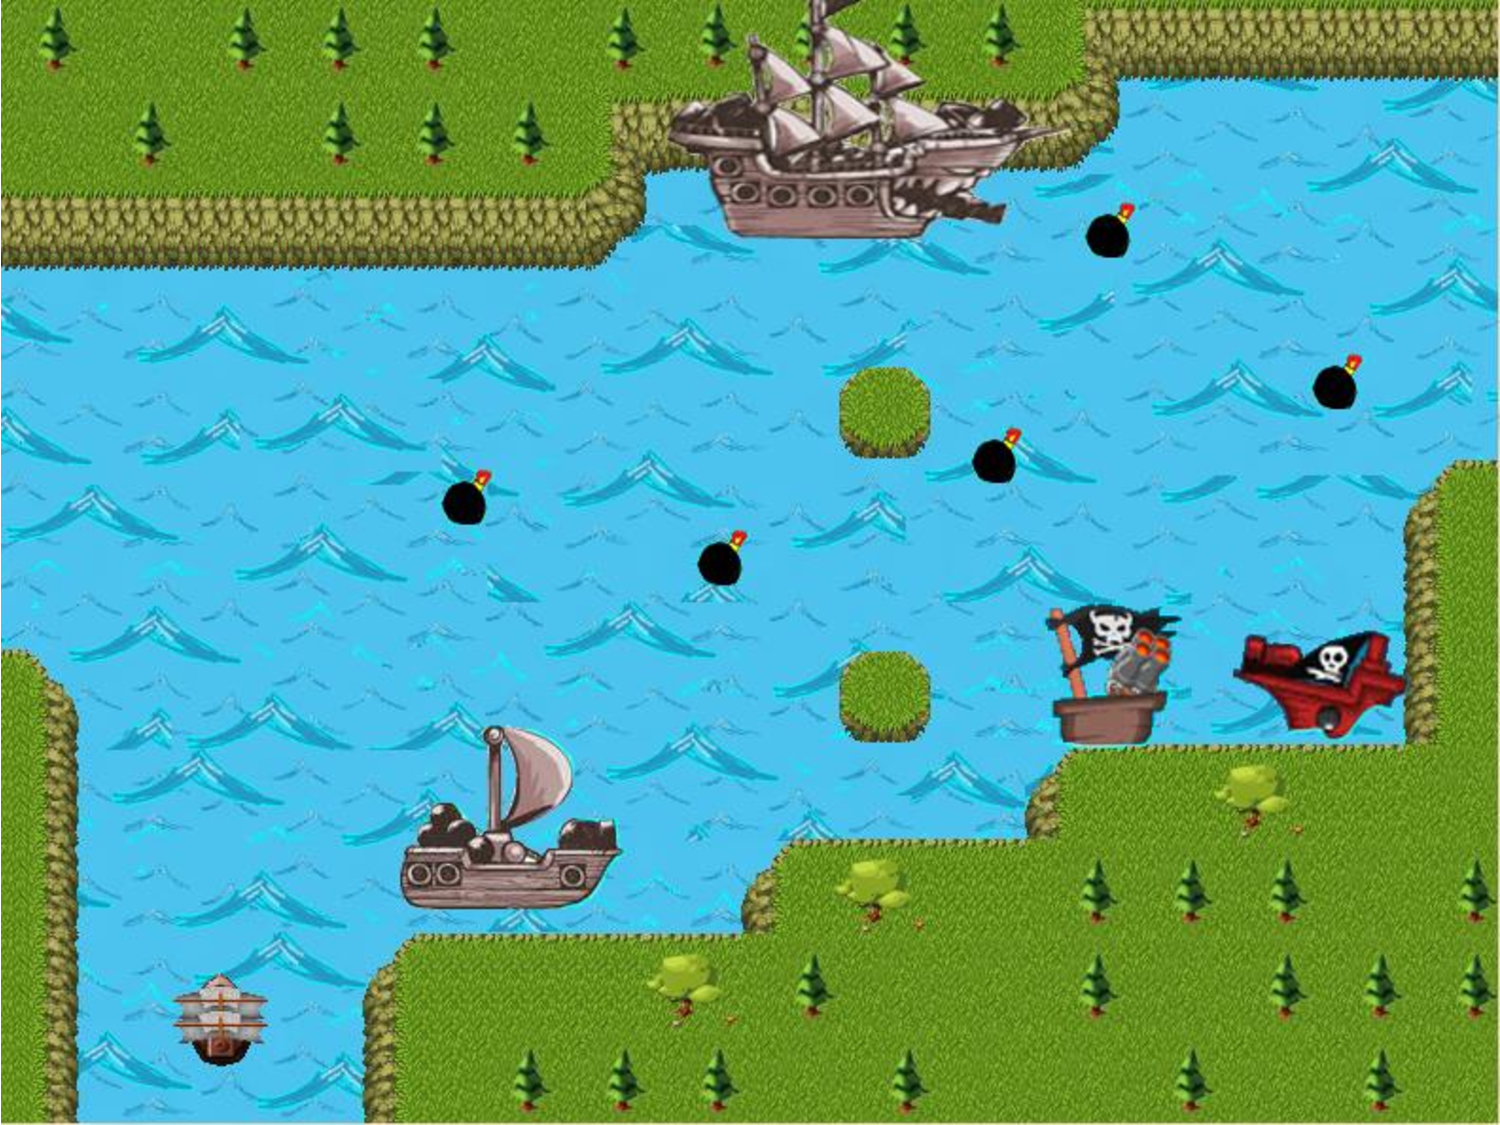
\includegraphics[scale=0.30]{img1.pdf}
\caption{Fase 1}
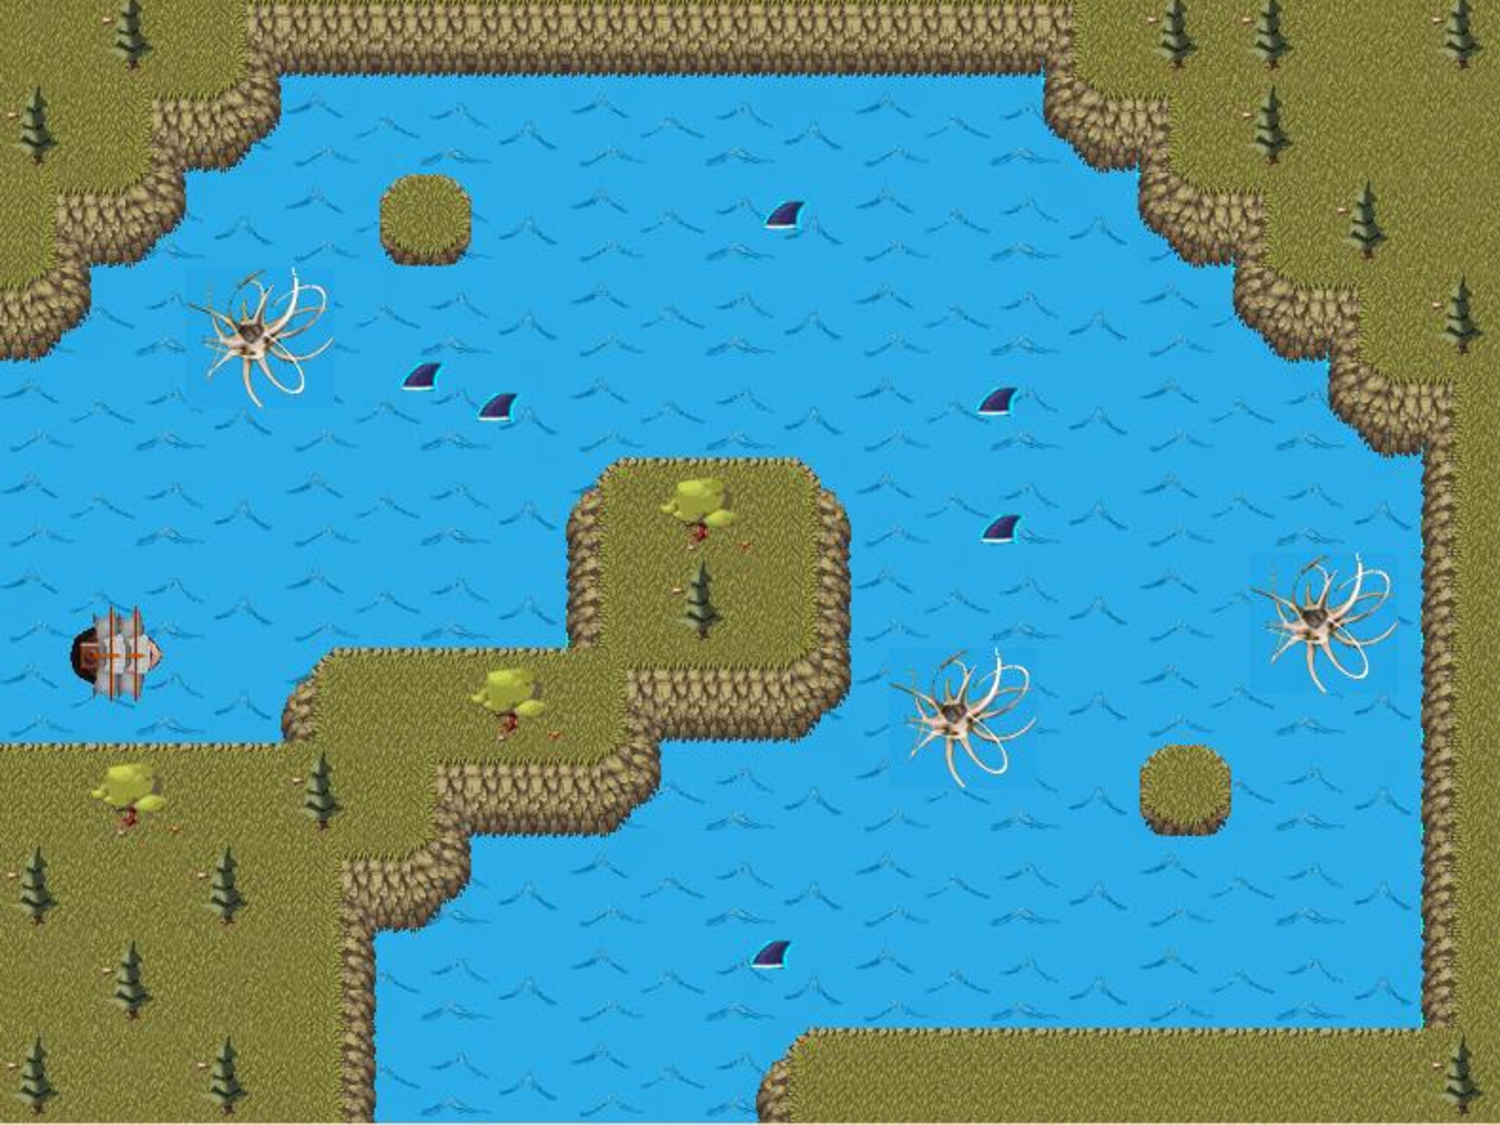
\includegraphics[scale=0.30]{img2.pdf}
\caption{Fase 2}
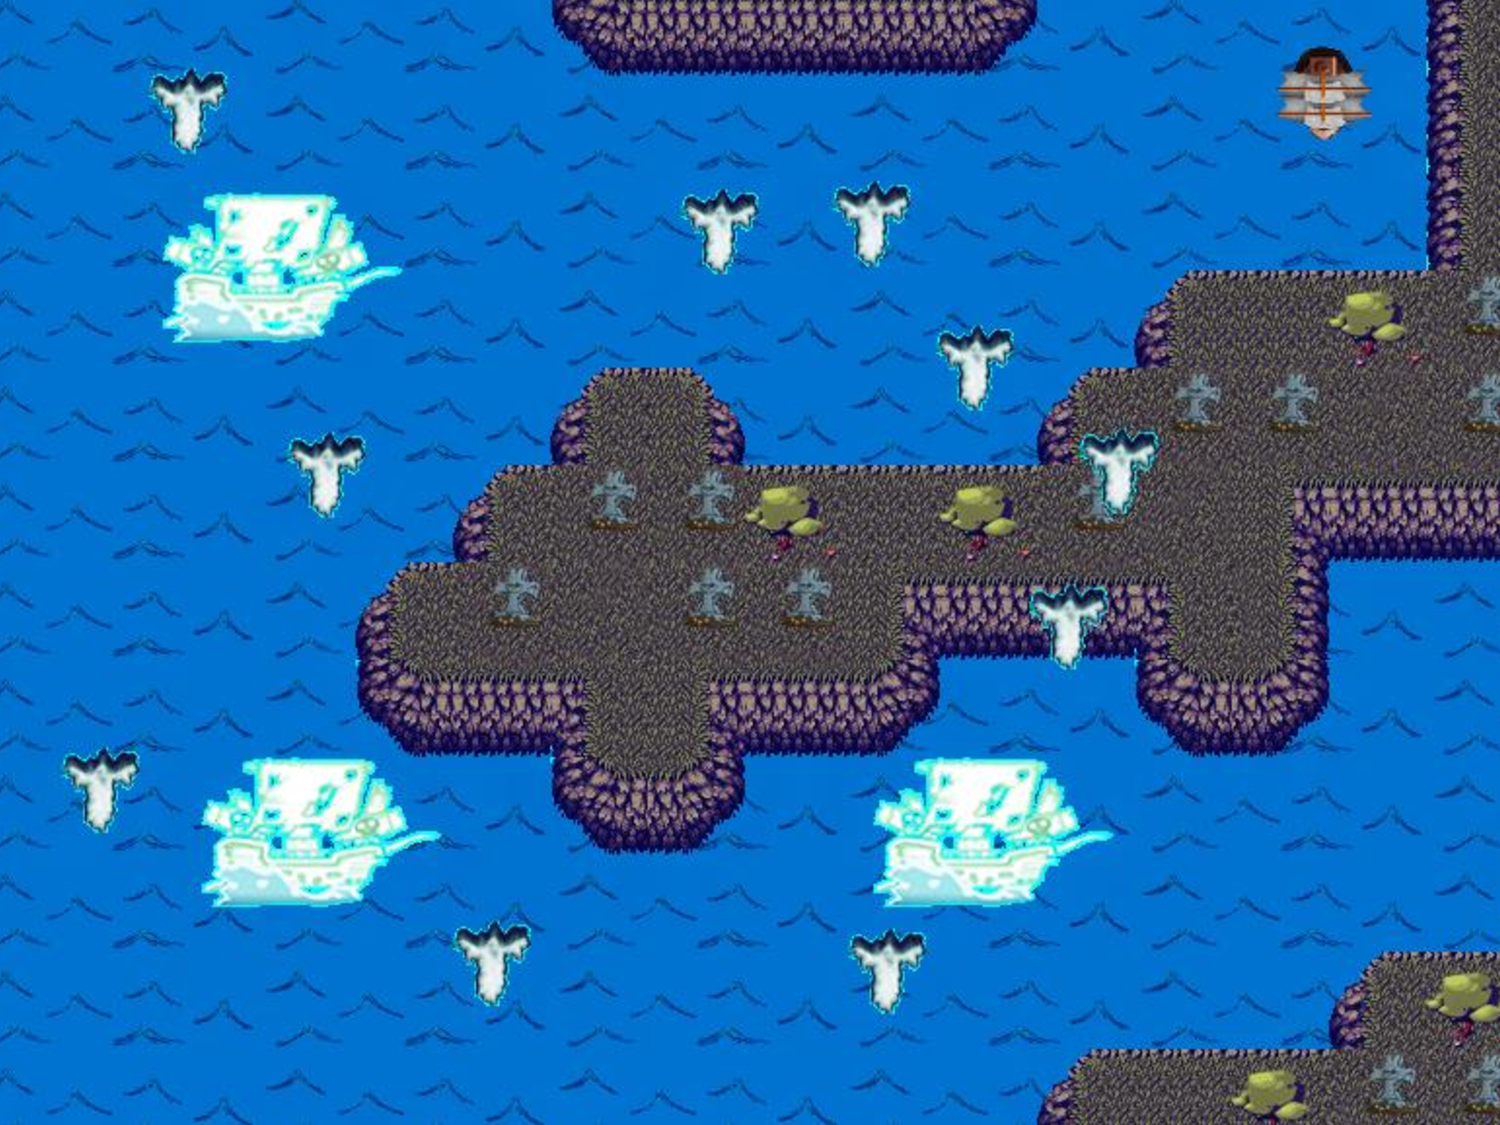
\includegraphics[scale=0.30]{img3.pdf}
\caption{Fase 3}
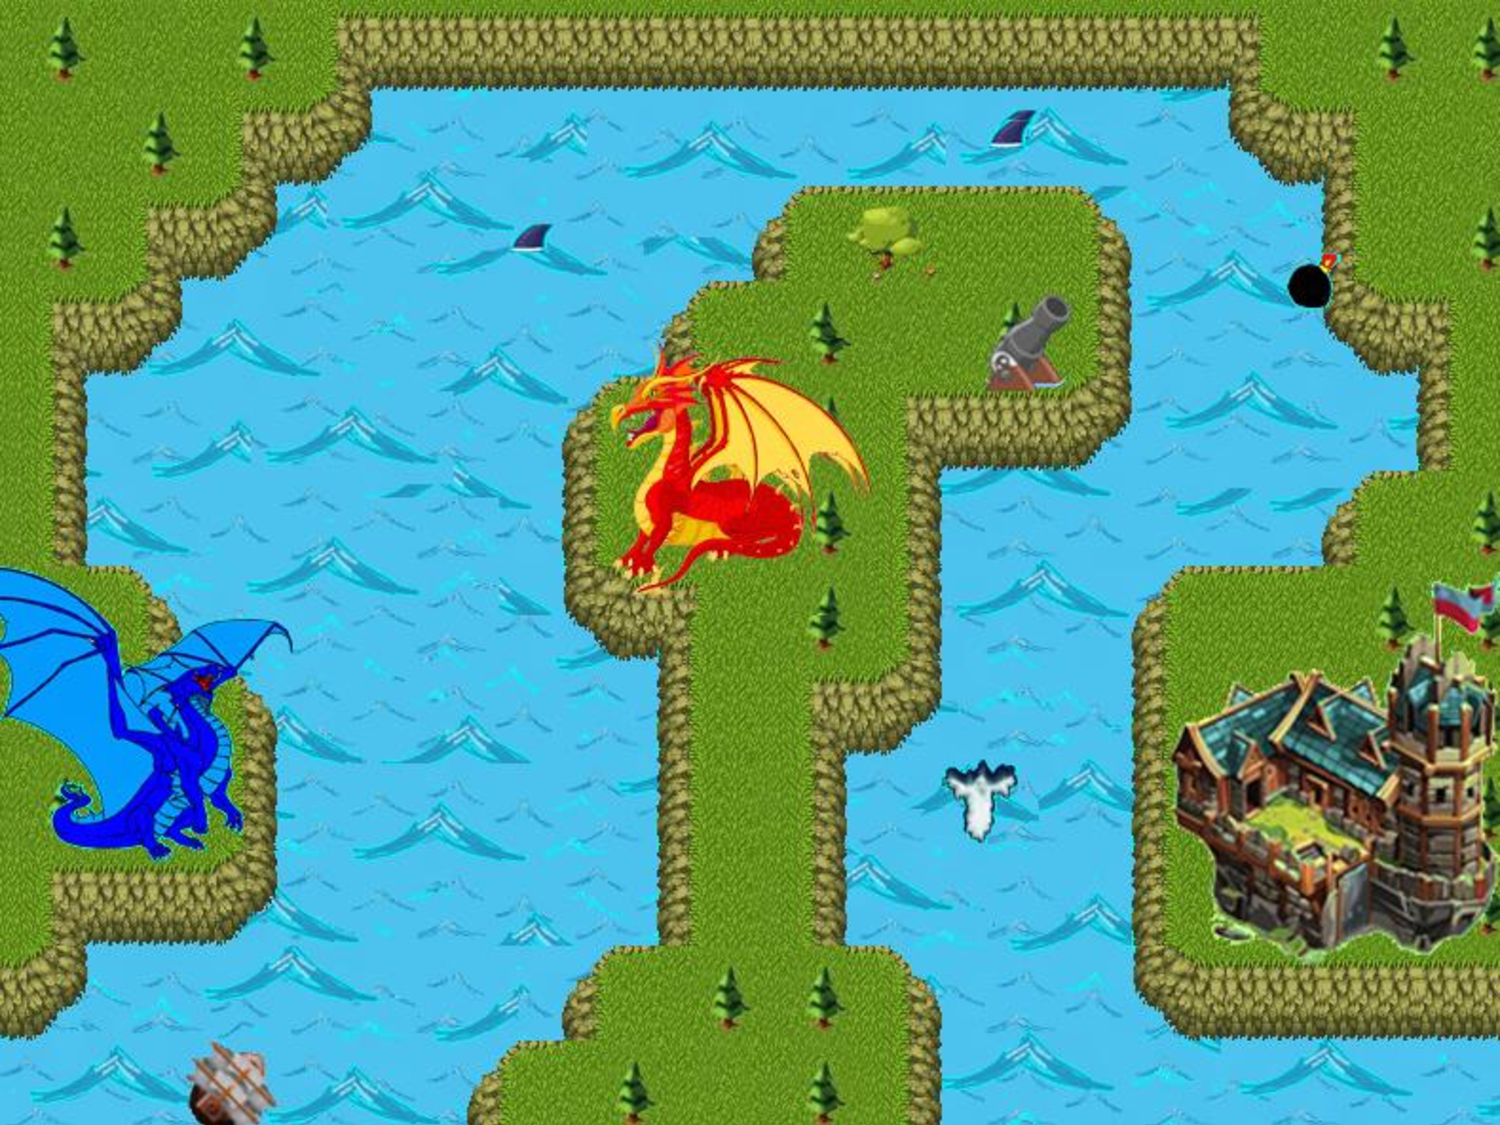
\includegraphics[scale=0.30]{img4.pdf}
\caption{Fase 4}
\end{center}
\end{figure}



\end{document}